\chapter{Opracowane algorytmy}
\label{c4}

\section{Wstęp}
\label{c41}
Poniższy rozdział poświęcono przedstawieniu idei, opisu i cech zaprojektowanych algorytmów. Oba oparte są na opisanych w poprzednim rozdziale algorytmach przetwarzania zbiorów zapytań eksploracyjnych, tj. Common Counting (\cite{WojciechowskiCC}) i Common Candidate Tree (\cite{WojciechowskiCCT}). Implementacja Apriori wykorzystywana wewnątrz tych algorytmów jest zgodna z rozwiązaniem zaproponowanym przez Borgelta (\cite{Borgelt}). 

\section{Przygotowanie danych}
\label{c42}
Zbiór danych, w którym poszukiwane są zbiory częste z użyciem Common Counting lub Common Candidate Tree musi spełniać kilka założeń. Krokiem wstępnym wykonania obu algorytmów jest zatem odpowiednie przygotowanie danych. Po pierwsze elementy każdej transakcji są sortowane leksykograficznie. Następnie niezbędne jest wyznaczenie zbioru elementarnych predykatów selekcji danych dla zbioru zapytań eksploracyjnych \(S = \{s_1, s_2, \dots, s_n\}\). Przykładowo jeżeli relacja \(R\) posiada atrybut całkowitoliczbowy \(a\) oraz do wykonania są trzy zapytania eksploracyjne \(dmq_1=(R, 0 \leq a < 10, \emptyset, 4\%)\), \(dmq_2=(R, 5\leq a < 20, \emptyset, 2\%)\), \(dmq_3=(R, 0\leq a < 5~or~25\leq a < 30, \emptyset, 3\%)\), to w tym wypadku zbiór elementarnych predykatów selekcji danych będzie równy  \(S = \{0\leq a < 5, 5\leq a < 10, 10\leq a < 20, 25\leq a < 30\}\). Znając ten zbiór można zdefiniować podzielić zbiór danych na rozłączne partycje i minimalizować ich odczyt. Dane odczytane z partycji są przetwarzane przez te zapytania, które się do niej odnoszą. Sprawia to, że części wspólne dla wielu zapytań są odczytywane tylko raz. Wejściem dla obu opracowanych algorytmów jest zbiór \(DMQ\).

\section{Struktura wierzchołka}
\label{c43}
Wierzchołek drzewa prefiksowego zbudowany w podobny sposób do tego zaproponowanego dla CC (\cite{WojciechowskiCC}) i CCT (\cite{WojciechowskiCCT}). Tzn. w przypadku Common Counting wierzchołek zawiera licznik wystąpień oraz listę elementów w zbiorze reprezentowanym przez ten wierzchołek, natomiast w przypadku Common Candidate Tree jest to wektor liczników (jego pola odpowiadają kolejnym zapytaniom eksploracyjnym, tj. \(i\)-ty element wektora, to licznik wystąpień danego zbioru dla \(dmq_i\)), wektor flag logicznych informujących, które zapytania odnoszą się do danego wierzchołka (zależność jak w przypadku liczników - \(i\)-ty element wektora informuje czy wierzchołek zawiera się w \(dmq_i\)). Dodatkowo w obu przypadkach dołożona została lista etykiet dla każdego wierzchołka. Etykiety odpowiadają wszystkim krawędziom wychodzącym z danego wierzchołka. Pozwala to na łatwiejsze i szybsze poruszanie się po drzewie podczas wykonywania na nim operacji. Struktura wierzchołka wykorzystywana w CCTP zaprezentowana została na rysunku \ref{fig:nodeCCTP}.
\begin{figure}[h]
	\centering
	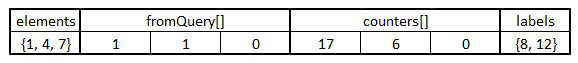
\includegraphics[width=0.8\linewidth]{figures/node}
	\caption{Struktura wierzchołka wykorzystywana w CCTP.}
	\label{fig:nodeCCTP}
\end{figure}

\section{Implementacja algorytmu Apriori}
\label{c44}

Implementacja Apriori zastosowanego wewnątrz CC i CCT jest inspirowana propozycją Borgelta \cite{Borgelt}. Zastosowane zostało drzewo prefiksowe jako struktura przechowująca kandydatów, dla których ustalane jest wsparcie. Drzewo generowane jest od korzenia. Na pierwszym poziomie znajdują się wszystkie możliwe zbiory jednoelementowe. Ich liczność odpowiada liczbie różnych elementów w zbiorze wszystkich elementów występujących w przetwarzanych transakcjach. Następnie wykonywane jest ustalanie wsparcia dla każdego wierzchołka. Kolejny poziom w drzewie generowany jest tylko z wierzchołków zawierających zbiory częste. Dzięki temu znacząco zmniejsza się rozmiar wygenerowanego drzewa. Dla pierwszego poziomu wsparcie jest po prostu sumą wystąpień poszczególnych elementów w transakcjach. Dla pozostałych poziomów Wsparcie wyznaczane jest metodą rekurencyjną liczenia rekurencyjnego (RC) (ang. \textit{recursive counting}). Metoda ta działa dla każdego wierzchołka w następujący sposób: (1) przejdź do dziecka wskazywanego przez krawędź z etykietą odpowiadającą pierwszemu elementowi transakcji i~przetwarzaj dla niego pozostałe elementy transakcji w ten sam sposób oraz (2) pomiń pierwszy element transakcji i~przetwarzaj dla danego wierzchołka pozostałe elementy. Gdy metoda znajdzie się na poziomie odpowiadającym aktualnie dodanym kandydatom, to zwiększany jest licznik wystąpień w danym wierzchołku i nie następuje dalsze przechodzenie w głąb drzewa. Procedura ta jest sekwencyjnie powtarzana dla każdej transakcji. Dodatkowo, w celu zmniejszenia liczby analizowanych transakcji, sprawdzane jest czy liczba elementów transakcji jest wystarczająca do osiągnięcia rozważanej głębokości drzewa - jeśli nie, to taka transakcja jest pomijana. Algorytm Apriori kończy się w~momencie gdy nie udało się wygenerować kandydatów dla kolejnego poziomu drzewa.

\section{Common Counting z wykorzystaniem drzew prefiksowych (CCP)}
\label{c45}
Pseudokod tej metody przedstawiono na Rysunku.~\ref{fig:CCFigure}. Odpowiada on temu co zostało zaproponowane w \cite{WojciechowskiCC} i opisane w punkcie \ref{c325}. Zmiana polega zastosowaniu adaptacji Apriori opisanej w sekcji \ref{c44}. W liniach 1-2 ustalane są wszystkie możliwe elementy i tworzoną one pierwszy poziom drzewa. Następnie ze zbiorów częstych o rozmiarze \(k-1\) generowane są \(k\)-elementowe zbiory kandydatów (dla \(k > 1\)). Jest to realizowane osobno dla każdego z zapytań \(dmq_i\) i~przebiega w~sposób opisany w \ref{c44}. Ostatnim krokiem jest zebranie odpowiedzi na zapytania eksploracyjne ze zbioru \(DMQ\) (linie 12-13). 

\begin{figure}[h]
	\noindent
	\hspace*{6em}\textbf{Input:} $ DMQ = \{dmq_1, dmq_2, ..., dmq_n\} $, \\
	\noindent
	\hspace*{6em}where $ dmq_i = (\mathcal{R}, a, \Sigma_i, \Phi_i, minfreq_i) $ \\
	\hspace*{6em} (1) \hspace{1em} \textbf{for} ($i$=1; $i \leq n$; $i$++) \textbf{do} \\
	\hspace*{6em} (2) \hspace{2em}   $\mathcal{C}_1^i$ = {all possible 1-itemsets} \\
	\hspace*{6em} (3) \hspace{1em} \textbf{for} ($k$=1; $\mathcal{C}_k^1 \cup \mathcal{C}_k^2 \cup..\cup \mathcal{C}_k^n \neq \emptyset$; $k$++) \textbf{do begin} \\
	\hspace*{6em} (4) \hspace{2em}   \textbf{for each} $s_j \in S$ \textbf{do begin} \\
	\hspace*{6em} (5) \hspace{3em}       $\mathcal{C}\mathcal{C}= \{\mathcal{C}_k^i : \sigma_{s_j}\mathcal{R}
	\subseteq \sigma_{\Sigma_i}\mathcal{R}\}$ \\
	\hspace*{6em} (6) \hspace{3em}       \textbf{if} $\mathcal{C}\mathcal{C} \neq \emptyset $
	\textbf{then} $ count(\mathcal{C}\mathcal{C}, \sigma_{s_j}\mathcal{R}) $ \textbf{end} \\
	\hspace*{6em} (7) \hspace{2em}    \textbf{for} ($i$=1; $i \leq n$; $i$++) \textbf{do begin} \\
	\hspace*{6em} (8) \hspace{3em}      $minsup_i = \lceil minfreq_i * |\sigma_{\Sigma_i}\mathcal{R}| \rceil$  \\
	\hspace*{6em} (9) \hspace{3em}      $\mathcal{F}_k^i = \{C \in \mathcal{C}_k^i : C.counter \geq minsup_i\} $ 	 \\
	\hspace*{6em} (10)\hspace{3em}      $\mathcal{C}_{k+1}^i = apriori\_gen(\mathcal{F}_k^i)$ \textbf{end} \\
	\hspace*{6em} (11)\hspace{1em} \textbf{end} \\
	\hspace*{6em} (12)\hspace{1em} \textbf{for} ($i$=1; $i \leq n$; $i$++) \textbf{do} \\
	\hspace*{6em} (13)\hspace{2em}    $Answer_i = \sigma_{\Phi_i} \bigcup_k \mathcal{F}_k^i$
	\caption{Pseudokod metody Common Counting}
	\label{fig:CCFigure}
\end{figure}


\section{Common Candidate Tree z wykorzystaniem drzew prefiksowych (CCTP)}
\label{c46}
Pseudokod tej metody przedstawiono na Rysunku.~\ref{fig:CCTFigure}. Pokrywa się on z tym co zostało zaproponowane w \cite{WojciechowskiCCT} i opisane w punkcie \ref{c326}. Zmiana polega zastosowaniu adaptacji Apriori opisanej w sekcji \ref{c44}, a co za tym idzie zmianie wykorzystywanej struktury z drzewa haszowego na prefiksowe, innym sposobie generowania kandydatów (linie 7-9) oraz wyznaczania ich wsparcia (linie 4-6) (zgodnie z tym co opisano w \ref{c44}). Podobnie jak w przypadku CCP ostatnim krokiem jest zebranie odpowiedzi na zapytania eksploracyjne ze zbioru \(DMQ\) (linie 12-13). Jednakże wykorzystywanie drzew prefiksowych wymaga utrzymania elementów wewnątrz wierzchołków drzewa w kolejności rosnącej. Ma to odzwierciedlenie w kroku generowania kandydatów, a dokładniej łączenia zbiorów kandydatów wygenerowanych przez wszystkie zapytania. Ostatecznie zdecydowano się na sprawdzanie kolejności elementów wewnątrz wierzchołka-kandydata podczas dodawania go do drzewa i~ewentualne sortowanie w przypadku gdy jest to konieczne. 
\begin{figure}[h]
	\noindent
	\hspace*{6em}\textbf{Input:} $ DMQ = \{dmq_1, dmq_2, ..., dmq_n\} $, \\
	\noindent
	\hspace*{6em}where $ dmq_i = (\mathcal{R}, a, \Sigma_i, \Phi_i, minfreq_i) $ \\
	\hspace*{6em} (1) \hspace{1em} $\mathcal{C}_1$ = {all possible 1-itemsets} \\
	\hspace*{6em} (2) \hspace{1em} \textbf{for} ($k$=1; $\mathcal{C}_k \neq \emptyset$; $k$++) \textbf{do begin} \\
	\hspace*{6em} (3) \hspace{2em}   \textbf{for each} $s_j \in S$ \textbf{do begin} \\
	\hspace*{6em} (4) \hspace{3em}       $\mathcal{C}\mathcal{C}= \{C \in \mathcal{C}_k : \exists i \; C.fromQuery[i] = true \wedge \sigma_{s_j}\mathcal{R}
	\subseteq \sigma_{\Sigma_i}\mathcal{R}\}$ \\
	\hspace*{6em} (5) \hspace{3em}       \textbf{if} $\mathcal{C}\mathcal{C} \neq \emptyset $
	\textbf{then} $ count(\mathcal{C}\mathcal{C}, \sigma_{s_j}\mathcal{R}) $ \textbf{end} \\
	\hspace*{6em} (6) \hspace{2em}    \textbf{for} ($i$=1; $i \leq n$; $i$++) \textbf{do begin} \\
	\hspace*{6em} (7) \hspace{3em}      $minsup_i = \lceil minfreq_i * |\sigma_{\Sigma_i}\mathcal{R}| \rceil$  \\
	\hspace*{6em} (8) \hspace{3em}      $\mathcal{F}_k^i = \{C \in \mathcal{C}_k : C.counters[i] \geq minsup_i\} $ 	 \\
	\hspace*{6em} (9) \hspace{3em}      $\mathcal{C}_{k+1}^i = apriori\_gen(\mathcal{F}_k^i)$ \textbf{end} \\
	\hspace*{6em} (10)\hspace{2em}    $\mathcal{C}_{k+1} = \mathcal{C}_{k+1}^1 \cup \mathcal{C}_{k+1}^2 \cup..\cup \mathcal{C}_{k+1}^n $ \\
	\hspace*{6em} (11)\hspace{1em} \textbf{end} \\
	\hspace*{6em} (12)\hspace{1em} \textbf{for} ($i$=1; $i \leq n$; $i$++) \textbf{do} \\
	\hspace*{6em} (13)\hspace{2em}    $Answer_i = \sigma_{\Phi_i} \bigcup_k \mathcal{F}_k^i$
	\caption{Pseudokod metody Common Candidate Tree}
	\label{fig:CCTFigure}
\end{figure}

Przykład uzasadniający dodatkowy krok algorytmu został zaprezentowany na rysunku \ref{fig:reorderProblem}. Jak widać w wyniku generowania kandydatów dla \(dmq_1\) powstał wierzchołek \(\{0, 1, 3\}\), następnie dla \(dmq_2\) utworzono \(\{0, 1, 2\}\) oraz ustawiono odpowiednią flagę \(fromQuery_2\) w wektorze flag wierzchołka \(\{0, 1, 3\}\). W wyniku generowania kolejnych kandydatów bez sortowania wartości zapytanie \(dmq_2\) wygenerowałoby wierzchołek \(\{0, 1, 3, 2\}\), co byłoby niezgodne z założeniami na temat drzewa prefiksowego. Dlatego też dla każdego dodawania sprawdzane są ostatnie dwa elementy i jeśli jest taka konieczność, to są one zamieniane miejscami. Pozostała część listy elementów jest wspólnym prefiksem i nie musi być weryfikowana.
\begin{figure}[h]
	\centering
	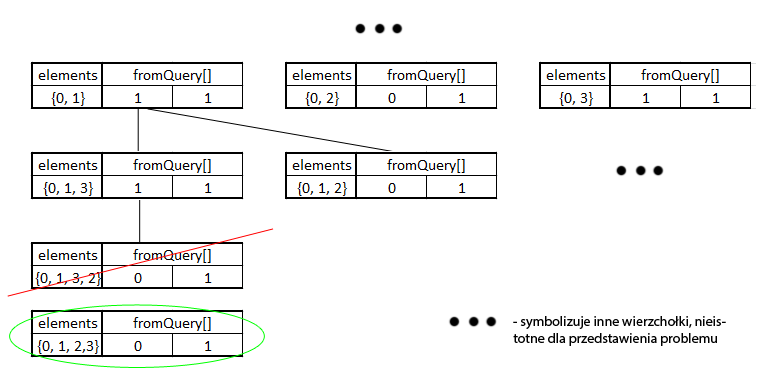
\includegraphics[width=0.8\linewidth]{figures/reorderProblem}
	\caption{Przykład uzasadniający konieczność sprawdzania elementów podczas dodawania wierzchołka.}
	\label{fig:reorderProblem}
\end{figure}

